\subsection{Data compression}

A "lossless" compression algorithm is defined as any coding procedure whose objective is to represent a certain quantity of information using or occupying a smaller space allowing the exact reconstruction of the original data.

\subsubsection{Introduction to Huffman's compression}

Invented by David Albert Huffman and published in 1952, Huffman coding is a lossless data compression algorithm. It uses a variable-length code to represent a symbol in the source message. The compressed binary code is determined by estimating the probability of occurrence of the symbols linked to the branches of a binary tree.

There are several implementations of this binary tree: \cite{wiki_huffman}

\begin{itemize}
 \item Static : Each byte has a predefined code, the tree does not need to be transmitted ;
 \item Semi-Adaptive : Calculates the occurrence of each byte, the tree needs to be transmitted ;
 \item Adaptive : Uses a known tree modified dynamically as the stream is compressed according to the symbols previously encountered ;
\end{itemize}

For the purposes of this report, we will be implementing the semi-adaptive

\subsubsection{Principles}age

The string we are going to compress is \textbf{"Information theory"}, and its binary code is as follows: \textbf{01001001 01101110 01100110 01101111 01110010 01101101 01100001 01110100 01101001 01101111 01101110 00100000 01110100 01101000 01100101 01101111 01110010 01111001}

Needless to say, it's a lot and that's why we're trying to compress it using our algorithm.
The principle is as follows: we calculate the occurrence of each letter in the source (the character string), then we sort this list in ascending order of occurrence. This list can be used to build a binary tree in the following "Bottom-Up" way:
\begin{figure}[H]
    \centering
    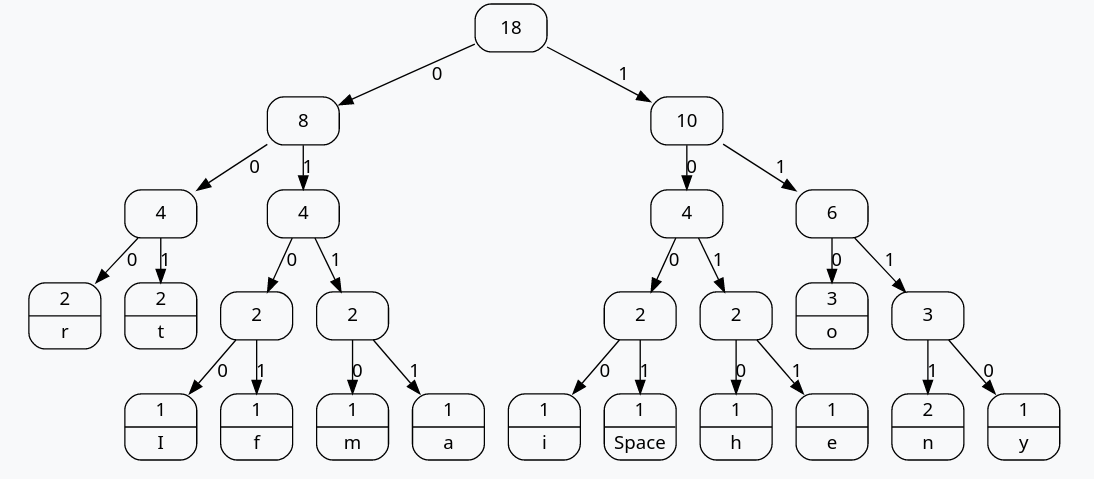
\includegraphics[width=0.5\linewidth]{images/HuffmanBT.png}
    \caption{Enter Caption}
    \label{fig:huffman-bt}
\end{figure}

By traversing this tree from node to node to reach the nodes corresponding to the letters we are looking for, we can find the compressed binary code assigned to them. The nodes on the left have a metric of 0 on their branch and a metric of 1 for the branches on the right (refer to the diagram of the previous tree). This gives the following binary code for the chosen source: \textbf{1101100100101110111101100100111011000011000000010111100} ... Much better, isn't it?

In order to decompress our compressed source and retrieve the exact starting data, we need to transmit the tree when communicating the source. (In Python we pass the object created for the tree).

As each node corresponds to a letter and has a weight on the branch linking it to other nodes, we can recover the exact source by simply traversing the tree and obtaining the \textbf{"Information theory"} string again.

\subsubsection{Limits and Performances}

For any source \textbf{X} with a Shannon entropy noted \textbf{H(X)} has an average length \textbf{L} of a codeword obtained by Huffman coding verified the following property: 

$H(X) <= L < H(X) + 1$.

The previous relationship shows that Huffman's algorithm approximates the entropy of our source and this may not be very interesting in the case of high entropy, where an overhead of 1 bit becomes significant. 

One solution to this problem is to work on blocks of \textbf{n} symbols. We then show that we can get closer to the entropy: 

$ H(X)\leq L<H(X)+{\frac {1}{n}} $

but the process of estimating probabilities becomes more complex and costly.